\clearpage{\pagestyle{empty}\cleardoublepage}
\chapter{Visualizzazione dati sull'utilizzo del progetto BolognaWiFi}
In questo capitolo andremo a trattare l'applicazione sviluppata, partendo da alcune considerazioni sui dati ufficiali forniti pubblicamente dal Comune di Bologna, per arrivare ad analizzare la struttura della stessa webapp.

Approfondiremo quindi i principali obiettivi, i problemi affrontati, le soluzioni implementate e l'ambiente di lavoro impiegato, per mostrare infine qualche schermata dell'applicazione così realizzata.

\section{Il caso studio: dati del BolognaWiFi}
% Descrizione del dataset, valore informativo, applicazioni per la pianificazione e gestione urbana
Il Comune di Bologna offre una serie di Open Data relativi al BolognaWiFi, riguardanti affollamento, affluenza e spostamenti, che vengono pubblicati ogni giorno mediante la rete Internet, in formato JSON. Il loro contenuto si riferisce a tutte le entrate giornaliere, riguardo alle varie zone e spostamenti, aggiornate a tre giorni prima della data odierna.

% Lo scopo della nostra applicazione è realizzare una visualizzazione dei dati in grado di mantenerne le informazioni sia a livello spaziale che temporale. Vedremo in seguito come siamo riusciti a sviluppare una tale dataviz e come il relativo sito degli Open Data non consenta una visualizzazione efficace dei dati.

Tutti questi dati sono stati aggregati in maniera oraria e anonima, quindi è impossibile risalire ai singoli dispositivi, rispettando così la privacy degli utenti. Tuttavia, la struttura dei dati non è omogenea in tutti e tre i dataset, quindi andremo a esplorarla nel dettaglio.

\subsection{Spostamenti}
Per gli spostamenti viene registrata una nuova entrata per ogni spostamento che viene effettuato in una data ora del giorno. Non è detto che ad ogni ora del giorno corrisponda almeno uno spostamento da una zona all'altra, in quanto non è detto che avvengano sempre, si pensi ad esempio durante le ore notturne.

\begin{figure}[H]
    \centering
    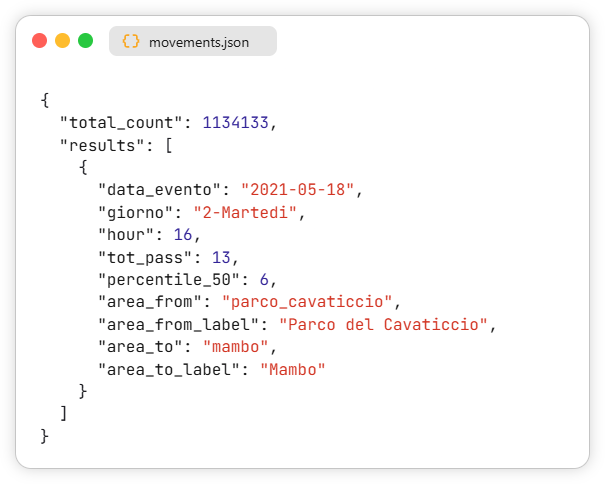
\includegraphics[width=\textwidth]{movements}
    \caption[Struttura dei dati sugli spostamenti]{Dati relativi agli spostamenti, in formato JSON, riferiti ai movimenti da Parco del Cavaticcio a Mambo, alle ore 16 del 18 maggio 2021.}
    \label{fig:movements}
\end{figure}

Tali spostamenti sono direzionati, quindi uno spostamento dalla Biblioteca Salaborsa a Palazzo D'Accursio verrà registrato separatamente da quello effettuato, inversamente, da Palazzo D'Accursio a Biblioteca Salaborsa. Anche in questo caso, entrambe le direzioni degli spostamenti sono indipendenti l'una dall'altra, e non è detto che esistano entrambe in una certa ora. Per esempio, potremmo avere una direzione in cui si spostano 100 persone (o meglio, dispositivi), mentre nell'altra se ne spostano 0 o comunque una quantità trascurabile ai fini del rilevamento dati di BolognaWiFi, quindi in entrambi questi ultimi due casi non verrebbe creata nessuna nuova entrata sul database di Open Data. Questo aiuta anche a garantire la privacy degli utenti, in quanto se venissero pubblicati i dati di un singolo dispositivo in una certa direzione il diritto alla privacy potrebbe venire violato.

\subsection{Affollamento e Affluenza}
Dato che affollamento e affluenza contengono dati aventi una struttura molto simile tra loro, possiamo trattarli insieme. Per entrambi viene registrata una nuova entrata per ogni ora del giorno, in ciascuna zona di Bologna coperta dal servizio BolognaWiFi.

\begin{figure}[H]
    \centering
    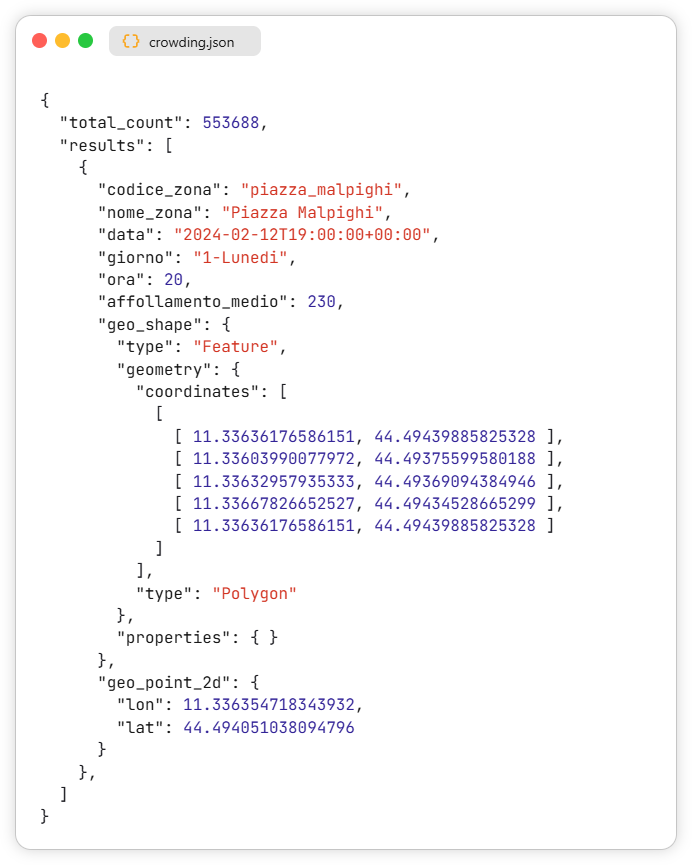
\includegraphics[width=\textwidth]{crowding}
    \caption[Struttura dei dati sull'affollamento]{Dati riguardanti l'affollamento, in formato JSON, riferiti a Piazza Malpighi alle ore 20 del 12 febbraio 2024. Notare l'attributo \textit{ora} che viene incluso nel timestamp di \textit{data} in fuso orario UTC.}
    \label{fig:crowding}
\end{figure}

\begin{figure}[H]
    \centering
    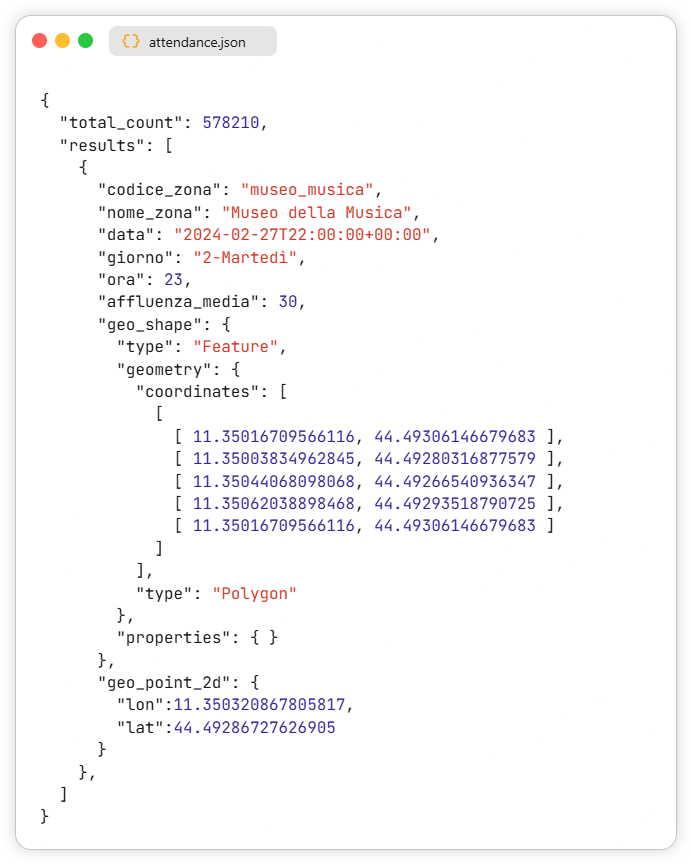
\includegraphics[width=\textwidth]{attendance}
    \caption[Struttura dei dati sull'affluenza]{Dati riguardanti l'affluenza, in formato JSON, riferiti al Museo della Musica, alle ore 23 del 27 febbraio 2024. Notare l'attributo \textit{ora} che viene incluso nel timestamp di \textit{data} in fuso orario UTC.}
    \label{fig:attendance}
\end{figure}

\section{Struttura del database}
La struttura dei dati ottenuti dall'interrogazione delle API, così come possiamo vedere in Figura~\ref{fig:movements}, Figura~\ref{fig:crowding} e Figura~\ref{fig:attendance}, è abbastanza semplice di per sé. Tuttavia, tale semplicità nasconde dei problemi di gestione delle ridondanze quando vengono salvati i dati su database, ciò avviene per svariati motivi che ora approfondiremo.

\subsection{Aree}
Innanzitutto, le informazioni relative alle aree e coordinate sono salvate in maniera differente nei tre dataset. Negli spostamenti si collegano solo i nomi e gli identificatori di ciascuna area attinente al vettore movimento, mentre sia in affollamento che in affluenza vengono specificate anche le relative coordinate del poligono, insieme a quelle del suo centroide.

Questo comporta fin da subito la necessità di creare un'entità per le aree e una separata per ciascuna coordinata, in quanto ogni poligono ha un numero variabile di punti. In questo modo non solo rimuoviamo la ridondanza tra affollamento e affluenza, ma permettiamo anche di collegare due poligoni a ciascuno spostamento, uno di partenza e uno di arrivo, cosa che non sarebbe possibile se non avessimo aggregato i tre dataset.

Notiamo subito che tale accortezza è possible solamente perché tutti e tre i dataset afferiscono alle stesse aree, ovvero i poligoni, delimitati dalla copertura del segnale di BolognaWiFi, quindi il loro dominio delle aree è completamente sovrapponibile.

\subsection{Spostamenti}
In questo modo, abbiamo assegnato un poligono di partenza e uno di arrivo a ciascuno spostamento. Rimane tuttavia il fatto che esista un numero \( n \) di spostamenti giornalieri, con \( n \leq 24 \), quindi al momento avremmo un numero esageratamente alto di entrate su database, che diventerebbe un problema in termini di richieste al server per visualizzare i dati giornalieri.

Questo problema può essere efficacemente risolto aggregando tutti i dati giornalieri: per fare ciò, fissata un'area di partenza e una di arrivo per una precisa data, creiamo 24 colonne per l'attributo \textit{percentile\_50} e altrettante 24 per \textit{tot\_pass}. In questo modo ottimizziamo il recupero dei dati effettuato dal client mediante richieste server, riducendo il numero di chiamate fino a 24 volte: basta semplicemente scaricare tutti i dati di un giorno, e utilizzarli fino a quando l'utente non chiama i dati di un altro giorno.

Riguardo al significato degli attributi, \textit{tot\_pass} è il numero di passeggeri che transitano da una zona A a una zona B nell'arco di un'ora in un determinato giorno. Invece, \textit{percentile\_50} è il mediano di tutti i \textit{tot\_pass} calcolati per tutti i giorni a una determinata ora, fino al giorno in cui vengono salvati i dati sul database di Open Data.

In questo caso, l'aggregazione dei dati è semplice perché nel dataset, nessun giorno ha un numero di entrate superiore a 24, cosa non scontata considerando che il cambio dell'ora genera un giorno con 23 ore in primavera e uno con 25 in autunno. Tale affermazione è affidabile in quanto la registrazione dei dati sugli spostamenti è cominciata l'1 aprile 2021.

\subsection{Affollamento e Affluenza}
Ancora una volta, questi due dataset si rivelano simili: avendo un insieme di attributi molto simili e lo stesso set di coordinate dei poligoni, basta scegliere uno qualunque dei due dataset per popolare le tabelle di area e coordinate che abbiamo visto prima.

In questo modo, entrambe le sezioni di \textit{geo\_shape} e \textit{geo\_point\_2d} vengono assorbite in area e coordinate, alleggerendo la struttura delle tabelle di affollamento e affluenza che andremo a realizzare. Possiamo notare che tutti i dati relativi ad affollamento e affluenza hanno un \textit{"type": "Feature"} e \textit{"type": "Polygon"}, che possono essere tranquillamente ignorati essendo uguali in tutto il dataset.

Anche qui, per ottimizzare le richieste al server nello stesso modo che abbiamo visto per gli spostamenti, aggreghiamo le 24 ore dello stesso giorno all'interno della stessa entrata, ma non solo: data la loro somiglianza, affollamento e affluenza possono essere aggregati all'interno della stessa tabella. Questo è possibile perché entrambe le loro entrate riguardano tutte le aree di Bologna ad ogni ora del giorno, quindi il numero totale è sempre uguale.

Tuttavia, in questo caso in entrambi i dataset vi sono giorni con 23 o 25 entrate giornaliere, a causa del cambio dell'ora. Tale problema si risolve facilmente, considerando che tutti gli eccessi hanno valori nulli: in caso di conflitto, basta tenere il valore massimo, in quanto uno dei due è per forza zero, mentre in caso di deficit basta assegnare 0 come valore al dato mancante.

Inoltre, sorge un ulteriore problema iniziale dovuto al fatto che i dati di affluenza sono disponibili a partire dal 1 gennaio 2024, mentre quelli riguardanti l'affollamento cominciano dal 15 gennaio 2024. Ancora una volta si risolve semplicemente assegnando uno 0 ai valori mancanti, ovvero a tutti quelli nelle due settimane in cui non vi sono dati riguardanti l'affollamento.

\subsection{Schema finale}
Dopo tutte le precedenti considerazioni, riportiamo in Figura~\ref{fig:database} lo schema finale del database. Per evitare di ottenere un database enorme in termini di spazio su disco, abbiamo prestato particolare attenzione ad utilizzare la quantità di memoria minore possibile per ogni attributo delle tabelle.

In particolare, considerando che gli spostamenti (sia totali che mediani), l'affollamento e l'affluenza orari raggiungono valori sempre interi che non superano mai la quantità di 10~000 e non sono mai inferiori a zero. Di conseguenza, possiamo utilizzare un tipo di dato \textit{unsigned short} senza avere timori relativi ad un possibile overflow, anzi possiamo mantenere pure una certa quantità di margine, occupando solo 2 bytes per numero, dimezzando lo spazio richiesto in confronto ai 4 bytes occupati da un normale \textit{unsigned int}.

Inoltre, una simile considerazione può essere effettuata per i numeri decimali relativi alle coordinate dei punti dei poligoni, in quanto vi sono sempre due cifre intere e 14 o 15 cifre decimali. Riguardo alle due cifre intere, possiamo utilizzarne sempre due solamente considerando la posizione geografica di Bologna, in quanto se la latitudine non rappresenta un problema, la longitudine talvolta può assumere valori a tre cifre intere in base alla posizione sulla Terra. In questo modo, su MySQL gli viene assegnato il tipo di dato \textit{decimal(17,15)}, con 15 cifre decimali su 17 cifre totali, escludendo la virgola.

\begin{figure}[H]
    \centering
    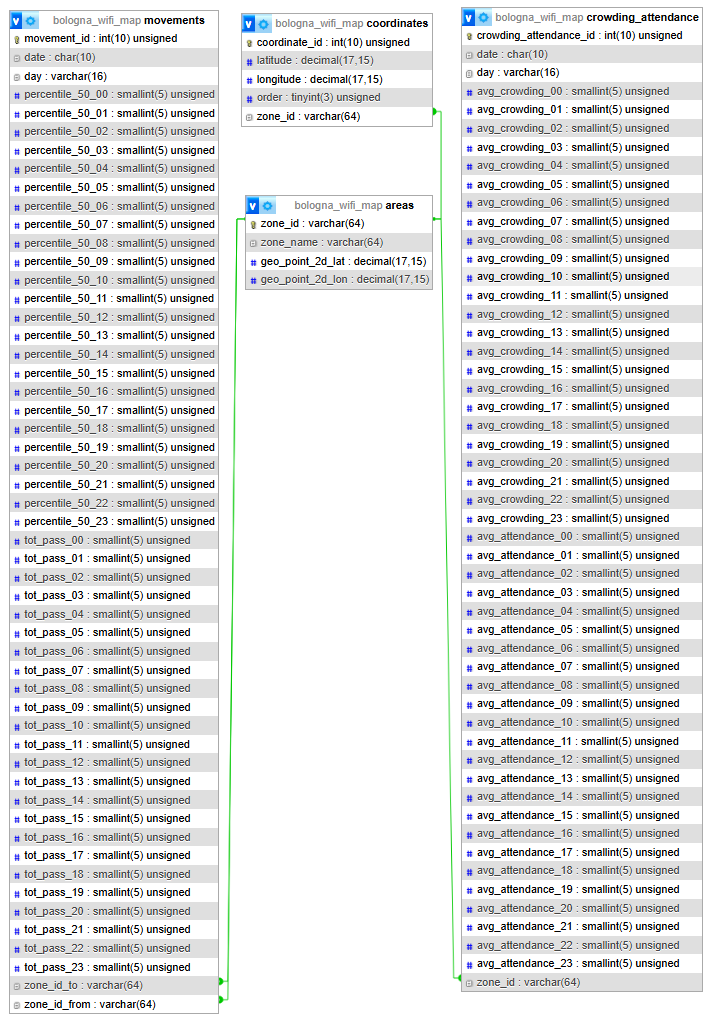
\includegraphics[width=\textwidth]{database.png}
    \caption[Schema del database]{Schema del database di BolognaWiFiMap. Notare la lista di attributi definiti per ciascuna ora.}
    \label{fig:database}
\end{figure}

\section{Connessione tra frontend e backend}
Dopo aver installato Vue.js e creato il progetto utilizzando Vite, ovvero un plugin di Vue per la nuova sintassi SFC (Single-File Components), abbiamo impostato l'indirizzo e la porta del server nel file di configurazione \Verb_vite.config.js_, settandolo a 0.0.0.0 per permettere al frontend di comunicare col backend indipendentemente dall'indirizzo del server, che in questo caso si riferisce a quello del server Apache. Inoltre, abbiamo specificato l'alias \Verb_@_ per definire la directory \Verb_./src/frontend_, semplificando il percorso dei file da importare.

\begin{figure}[H]
    \centering
    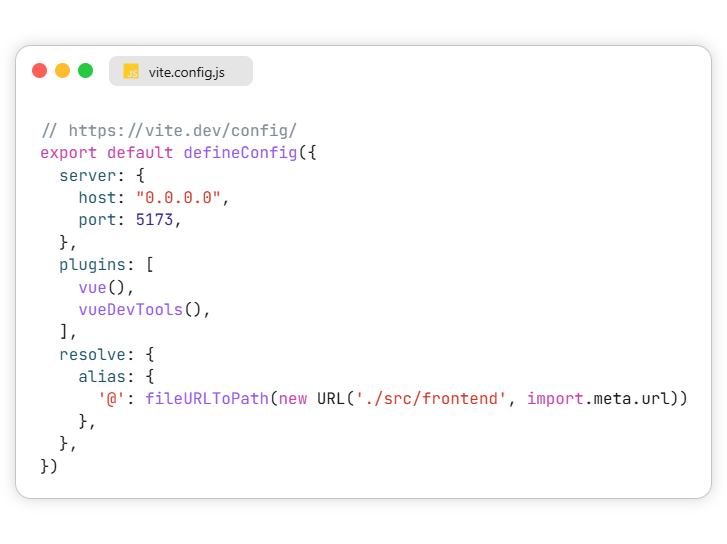
\includegraphics[width=\textwidth]{vite_config}
    \caption[Configurazione delle impostazioni Vite]{Configurazione delle impostazioni Vite relative al progetto Vue, dove si definiscono in particolare l'indirizzo e la porta per accedere al server.}
    \label{fig:vite_config}
\end{figure}

\section{Single-Page App}
Questa applicazione è stata realizzata seguendo il modello della \textit{Single-Page App}, ovvero una sola pagina web che carica selettivamente i suoi componenti o aggiorna i suoi dati senza necessità di ricaricare la pagina. Questo è permesso sia dallo stesso framework Vue.js, sia dall'implementazione di richieste AJAX che il client effettua al server.

\section{Implementazione richieste AJAX}
Le richieste AJAX sono effettuate in modo asincrono dal client al server per ottenere dei dati che verranno utilizzati per aggiornare la pagina, evitando di dover effettuare un ricaricamento della stessa. Per la sua implementazione abbiamo utilizzato la funzione \Verb_fetch()_ built-in di JavaScript, creando tre funzioni per aggiornare rispettivamente le aree, con \Verb_fetchAreas()_, gli spostamenti, con \Verb_fetchMovements()_, e infine l'affollamento insieme all'affluenza, con \Verb_fetchCrowdingAttendance()_. 

Abbiamo definito tutte queste funzioni nel file \Verb_api.js_, essendo molto semplici riportiamo in Figura~\ref{fig:ajax_api_movements} solo quella relativa agli spostamenti. In particolare, queste custom API utilizzano l'indirizzo corrente comprensivo di porta, per poi appendere a tale stringa l'url specifico dell'API a cui si vuole effettuare la richiesta. Si noti come questo setup presuppone un deployment di frontend e backend sullo stesso server, o quantomeno di un ridirezionamento tramite proxy di tali richieste effettuate a frontend verso l'url appropriato del backend, se dovessero essere in deployment su server diversi.

\begin{figure}[H]
    \centering
    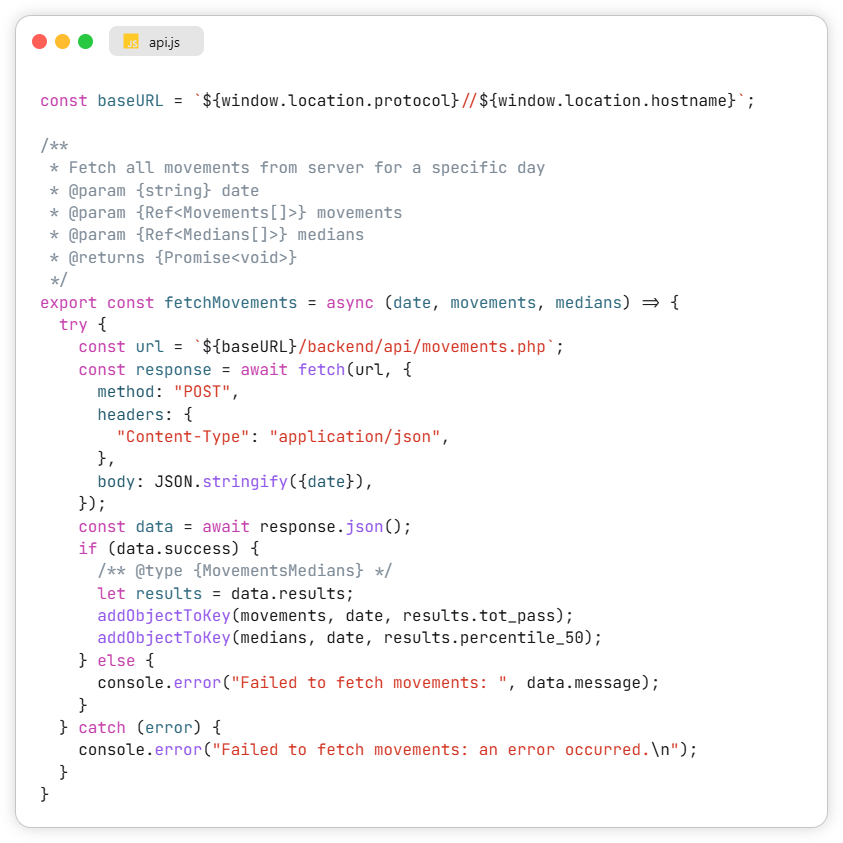
\includegraphics[width=\textwidth]{ajax_api_movements}
    \caption[Funzione AJAX per ottenere la lista dei movimenti di una specifica data]{Implementazione di una funzione che effettua una richiesta AJAX per ottenere la lista dei movimenti di una specifica data.}
    \label{fig:ajax_api_movements}
\end{figure}

\section{Popolamento del database}
Affinché le richieste AJAX possano andare a buon fine, bisogna aver popolato il database. Questo compito è svolto mediante l'esecuzione del file \Verb_updater.php_, il quale controlla l'ultima data dei dati raccolti sul database e provvede ad aggiornarli, scaricando tutti i nuovi dati.

In fase di development o test, questo script viene lanciato manualmente, ma in un futuro deployment basterebbe automatizzare la sua esecuzione utilizzando Task Scheduler su Windows o un Cron Job su Linux. Tale script, riportato in Figura~\ref{fig:updater} richiama 3 funzioni differenti per svolgere il suo compito, che qui non mostreremo per via della loro lunghezza.

\begin{figure}[H]
    \centering
    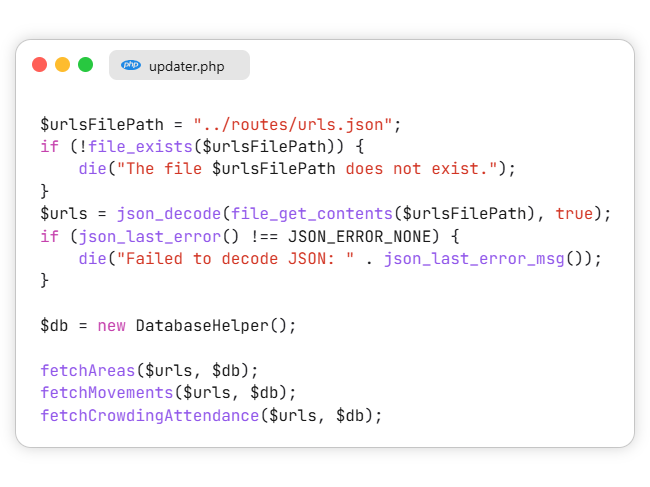
\includegraphics[width=\textwidth]{updater_noligature}
    \caption[]{Script che viene eseguito per effettuare il setup o per aggiornare i dati sul database, utilizzando gli url definiti in \textit{urls.json} per effettuare le chiamate alle API del sito degli Open Data di BolognaWiFi \cite{BolognaWiFi_Spostamenti,BolognaWiFi_Affollamento,BolognaWiFi_Affluenza}.}
    \label{fig:updater}
\end{figure}

Innanzitutto, viene aggiornata la lista delle aree, nel caso se ne trovino di nuove. Quindi si scaricano, in ordine, prima i movimenti, poi l'affollamento insieme all'affluenza. All'interno di entrambe le funzioni, vengono scaricati i dati giorno per giorno, fino ad arrivare agli ultimi disponibili. Tuttavia, date le limitazioni delle API offerte da BolognaWiFi, vengono scaricati al massimo 100 elementi alla volta. Questo chunk così ottenuto viene messo in coda in una lista, per poi effettuare una nuova chiamata alla stessa API riguardante lo stesso giorno, ma con un offset aumentato di 100. Le stesse API pongono un limite totale di 10~100 alla somma di offset e numero di elementi, ma considerando che in un singolo giorno non si arriva nemmeno a 2~000 elementi totali in tutti e tre i dataset, tale limite effettivo di 10~000 all'offset non è poi così restrittivo.

% \section{Funzionalità}
\section{Pagina iniziale}
Appena caricato il sito, viene visualizzata la mappa della città di Bologna insieme a tutte le aree coperte dal servizio BolognaWiFi, evidenziate come dei poligoni colorati in azzurro. Tali poligoni sono interattivi e, cliccandoli, viene mostrato un popup contenente il nome dell'area in questione. Inoltre, dato che queste aree variano molto in termimi di dimensioni, 

\section{Informazioni su una zona o spostamento}
\section{Calcolo del colore di una zona}
\section{Raggruppamento dei dati giornalieri}
\section{Analisi sull'usabilità}
% 2-3 task da fare valutare agli utenti se è più facile usare il mio sistema rispetto al sito degli open data + questionario SUS
% TASK:
% - visualizzazione delle zone coperte da segnale
% - visualizzazione spostamenti degli utenti tra le varie zone
% - visualizzazione di affollamento/affluenza di una specifica zona

% OPINIONI UTENTI: in forma anonima, basta una descrizione generale sui dati aggregati
% Dati in forma aggregata, specificando il range di valori per le informazioni anagrafiche e.g. età, per il SUS invece valore medio, min e max con dettaglio per risposta.

Una volta realizzata l'applicazione web, abbiamo reclutato un gruppo di utenti affinché svolgessero un test relativo all'usabilità, confrontando il sito degli Open Data con quello da noi realizzato, ovvero BolognaWiFiMap.

Innanzitutto, dobbiamo fare qualche considerazione sul campione di utenti preso in esame, avente dimensione \( n = 9 \), con \( n \) numero di utenti. Questo campione è indubbiamente piccolo, ma sufficiente a trarre le conclusioni necessarie alla valutazione della qualità del sistema realizzato.

Riguardo all'età degli utenti, questa varia in un range tra 23 e 30 anni (media 24.7, mediana 24.0). Stiamo quindi considerando un campione abbastanza uniforme di persone giovani e aventi familiarità con il mondo digitale. L'ultima considerazione è importante perché ci permette di imputare eventuali problemi alla scarsa usabilità del sito stesso e non a una bassa capacità di interazione digitale, e viceversa rende possibile capire se un sito sia ben utilizzabile.

\subsection{Feedback utente su task assegnati}
Per effettuare questo test in maniera standardizzata, abbiamo definito qualche task da sottoporre agli utenti. Tali compiti sono mirati a valutare la facilità di utilizzo dell'applicazione e riguardano i seguenti aspetti:
\begin{itemize}
    \item Visualizzazione delle zone coperte da segnale.
    \item Visualizzazione degli spostamenti degli utenti tra le varie zone.
    \item Visualizzazione dell'affollamento di una specifica zona.
    \item Visualizzazione dell'affluenza di una specifica zona.
\end{itemize}

Gli utenti dovevano valutare se fosse più facile svolgere questi compiti sul sito degli Open Data o se, al contrario, risultasse più comoda l'applicazione BolognaWiFiMap realizzata da noi. Dopodiché avrebbero lasciato un feedback che sarebbe stato raccolto in maniera anonima.

Per evitare di influenzare l'opinione degli utenti, abbiamo lasciato che svolgessero il test in totale autonomia, spiegando loro in maniera chiara quali fossero gli obiettivi sui quali focalizzarsi. Al fine di fornire agli stessi una comprensione di base sugli argomenti trattati da entrambi i siti, abbiamo spiegato concisamente agli utenti i concetti di BolognaWiFi, affollamento, affluenza e spostamenti, in modo da evitare un bias sui dati dovuto a una conoscenza inesistente dell'ambiente di test.

Le nostre aspettative iniziali ritenevano il sito degli Open Data più difficile da utilizzare rispetto al nostro sistema, e abbiamo in seguito avuto conferma dalle opinioni degli utenti che tali supposizioni erano assolutamente fondate, trovando un certo livello di consistenza all'interno dei feedback forniti. Andiamo quindi ad illustrare le opinioni degli utenti relative ai due sistemi.

\subsubsection{Open Data}
% Eu: assolutamente poco pratico, però ti dice letteralmente quello che è. Non ci si potrebbe mai fare un qualcosa di comodo e vendibile a delle persone, o comunque pratico.
% Mancu: "mi sento meno gay", fa schifo in confronto al mio
% Jyulo: "esperienza assolutamente anonima" perché cercava un modo carino per dire "non ho assolutamente capito un cazzo di quello che c'è in sto sito". Immaginava cosa fosse perché glielo avevo anticipato, ma altrimenti non ne aveva assolutamente idea perché "non si capisce un cazzo". Non sa se in quel sito lì uno ci va apposta perché ci vuole andare o se ci capita per caso reindirizzato da qualche parte, in quel caso è comunque un sito assolutamente inutile e non ha senso.
Le opinioni riguardanti il sito degli Open Data sono state prevalentemente negative. 7 utenti su 9 lamentavano il fatto che l'esperienza risultasse scarsissima, confusionaria e di difficile comprensione, con un utente che l'ha definita come assolutamente anonima. Tuttavia, 2 di questi 7 utenti hanno comunque sottolineato che, benché la scarsa praticità di utilizzo, questo sito rimanga comunque utile come banca dati. Gli altri due utenti hanno invece ritenuto la loro esperienza buona o addirittura ottima.

\subsubsection{BolognaWiFiMap}
% Eu: non è difficile ma è poco intuitivo: sarebbe da rendere solo un pochino più intuitivo.
% Mancu: la mappa è un po' strana ma va beh. Molto più facile da utilizzare
% Jyulo: gran bel sito
Riguardo al nostro sito BolognaWiFiMap, invece, le opinioni si sono radicalmente capovolte. Tutti gli utenti hanno evidenziato che l'esperienza risultasse buona o ottima, con un utente che è arrivato addirittura a definirla eccellente. Inoltre, sono rimasti tutti concordi sul fatto che questo sito sia molto più facile da utilizzare rispetto a quello degli Open Data. A vari livelli, la visualizzazione dei dati è stata ritenuta rapida e intuitiva, molto efficace a livello visivo. Solo un utente ha consigliato che potrebbe essere una buona idea rendere il sito ancora più intuitivo, offrendo spiegazioni ulteriori riguardo ai vari tipi di visualizzazioni di dati, seppur rimanendo dell'idea che già ora il sito sia facilmente utilizzabile. Quest'ultimo feedback fornisce uno spunto per un possibile sviluppo futuro dell'applicazione, volto a garantirne un'ancora maggiore accessibilità.

\subsection{Questionario SUS}
Ottenere un feedback dagli utenti è un ottimo passo in avanti per definire possibili punti di forza e debolezze di un'applicazione, ma queste opinioni hanno una natura prettamente soggettiva. Serve quindi un modo per valutare l'usabilità di un sistema in maniera standardizzata e il più obiettiva possibile, ed è qui che entra in gioco il questionario SUS.

Il questionario SUS (\textit{System Usability Scale}) è un insieme di 10 domande di carattere generale che possono essere utilizzate per valutare l'usabilità di un qualsiasi sistema su una scala da 0 (usabilità percepita molto scarsa) a 100 (usabilità percepita eccellente) \cite{SUS}.

Questo generalismo rappresenta il suo punto di forza, in quanto è in grado di adattarsi a qualunque tipo di applicazione, ma costituisce anche la sua più grande debolezza, dato che non permette di capire su quali aree lavorare per poter migliorare l'usabilità \cite{SUS}.

All'interno delle 10 domande, quelle dispari hanno una formulazione positiva e servono a calcolare la facilità d'uso, mentre quelle pari sono formulate in modo negativo appositamente per calcolare le possibili difficoltà legate all'utilizzo, contrastando con la domanda appena posta in precedenza.

Il punteggio finale del questionario SUS viene calcolato utilizzando la formula seguente \eqref{eq:sus_original} \cite{SUS_DesignersItalia}:

\begin{equation}
    SUS = \left( \sum_{i=1,3,5,7,9} (X_i - 1) + \sum_{i=2,4,6,8,10} (5 - X_i) \right) \times 2.5
    \label{eq:sus_original}
\end{equation}

Dove \( X_i \) sono le domande \( X_1, ..., X_{10} \). Quest'ultima formula può essere semplificata nella seguente \eqref{eq:sus_simplified} \cite{SUS_Wikipedia}:

\begin{equation}
    SUS = 2.5 \times \left( 20 + \sum_{i=1,3,5,7,9} X_i - \sum_{i=2,4,6,8,10} X_i \right)
    \label{eq:sus_simplified}
\end{equation}

La quale, a sua volta, può essere riscritta in forma abbreviata \eqref{eq:sus_shortened} per ottenere una maggiore chiarezza ed efficacia di comprensione \cite{SUS_Wikipedia}:

\begin{equation}
    SUS = 2.5 \times \left( 20 + \sum (\text{SUS}_{\text{odd}}) - \sum (\text{SUS}_{\text{even}}) \right)
    \label{eq:sus_shortened}
\end{equation}

Diventa ora chiaro dalla \eqref{eq:sus_shortened} come le domande dispari, positive, contribuiscano ad aumentare il punteggio finale del SUS, mentre quelle pari, negative, lo diminuiscano. Di conseguenza, è auspicabile che gli utenti rispondano con un voto alto alle domande dispari e con uno basso per quelle pari, al fine di ottenere un punteggio elevato.

Il questionario SUS che abbiamo sottoposto agli utenti è quello fornito da Designers Italia \cite{SUS_DesignersItalia}, ma la struttura del questionario è standardizzata in tutte le lingue. Di seguito elenchiamo la lista delle domande in Tabella~\ref{tab:sus_questions}.

\begin{center}
    \begin{table}[H]
        \centering
        \begin{tabularx}{1.02\textwidth}{|c|X|}
            \hline
            \multicolumn{2}{|c|}{\textbf{Questionario SUS}} \\
            \hline
            \textbf{Domanda} & \textbf{Descrizione}\\
            \hline
            SUS01 & Penso che mi piacerebbe utilizzare questo sito frequentemente.\\
            SUS02 & Ho trovato il sito inutilmente complesso.\\
            SUS03 & Ho trovato il sito molto semplice da usare.\\
            SUS04 & Penso che avrei bisogno del supporto di una persona già in grado di utilizzare il sito.\\
            SUS05 & Ho trovato le varie funzionalità del sito bene integrate.\\
            SUS06 & Ho trovato incoerenze tra le varie funzionalità del sito.\\
            SUS07 & Penso che la maggior parte delle persone possano imparare ad utilizzare il sito facilmente.\\
            SUS08 & Ho trovato il sito molto difficile da utilizzare.\\
            SUS09 & Mi sono sentito a mio agio nell'utilizzare il sito.\\
            SUS10 & Ho avuto bisogno di imparare molti processi prima di riuscire ad utilizzare al meglio il sito.\\
            \hline
        \end{tabularx}
        \caption[Lista di domande del questionario SUS]{Lista di domande del questionario SUS.}
        \label{tab:sus_questions}
    \end{table}
\end{center}

A ciascuna di queste domande, a prescindere se sia pari o dispari, si può rispondere con un numero intero da 1 (fortemente in disaccordo) a 5 (fortemente d'accordo). Quindi, non solo la formulazione delle domande è semplice, ma lo è altrettanto la valutazione delle relative risposte.

D'ora in poi, eviteremo di riportare nuovamente la descrizione per ogni domanda, ma ci riferiremo ad esse tramite la sigla SUS01 per la prima domanda, e così via.

\subsection{Risposte al questionario SUS}
Andiamo ora ad analizzare le risposte fornite dagli utenti. Riporteremo dapprima ciascuna delle due tabelle con i risultati individuali degli utenti, sia per il sito degli Open Data in Tabella~\ref{tab:sus_opendata}, sia per il nostro sito BolognaWiFiMap in Tabella~\ref{tab:sus_bolognawifimap}. Infine, mostreremo la Tabella~\ref{tab:sus_avg_values} contenente la media dei risultati per ciascuna domanda.

\begin{center}
    \begin{table}[H]
        \centering
        \begin{tabularx}{\textwidth}{|c|c|c|c|c|c|c|c|c|c|X|}
            \hline
            \multicolumn{11}{|c|}{\textbf{Risposte SUS Open Data}} \\
            \hline
            \textbf{S01} & \textbf{S02} & \textbf{S03} & \textbf{S04} & \textbf{S05} & \textbf{S06} & \textbf{S07} & \textbf{S08} & \textbf{S09} & \textbf{S10} & \textbf{SUS} \\
            \hline
            1 & 4 & 2 & 4 & 3 & 4 & 2 & 4 & 1 & 4 & 22.5 \\
            4 & 4 & 2 & 3 & 3 & 4 & 5 & 4 & 1 & 3 & 42.5 \\
            3 & 3 & 3 & 4 & 5 & 2 & 4 & 2 & 3 & 3 & 60.0 \\
            2 & 2 & 3 & 3 & 3 & 2 & 4 & 2 & 3 & 1 & 62.5 \\
            1 & 5 & 1 & 4 & 1 & 4 & 2 & 2 & 2 & 1 & 27.5 \\
            3 & 2 & 4 & 2 & 4 & 1 & 5 & 2 & 5 & 1 & 82.5 \\
            1 & 2 & 3 & 5 & 2 & 4 & 1 & 4 & 2 & 4 & 25.0 \\
            4 & 2 & 3 & 4 & 5 & 2 & 3 & 3 & 5 & 2 & 67.5 \\
            1 & 4 & 2 & 3 & 1 & 3 & 1 & 4 & 1 & 3 & 22.5 \\
            \hline
        \end{tabularx}
        \caption[Risposte del questionario SUS sul sito degli Open Data]{Risposte fornite dagli utenti sul questionario SUS relativo al sito degli Open Data, in forma anonima. Per motivi di spazio, i nomi delle domande sono stati abbreviati da SUS01 a S01.}
        \label{tab:sus_opendata}
    \end{table}
\end{center}

\begin{center}
    \begin{table}[h]
        \centering
        \begin{tabularx}{\textwidth}{|c|c|c|c|c|c|c|c|c|c|X|}
            \hline
            \multicolumn{11}{|c|}{\textbf{Risposte SUS BolognaWiFiMap}} \\
            \hline
            \textbf{S01} & \textbf{S02} & \textbf{S03} & \textbf{S04} & \textbf{S05} & \textbf{S06} & \textbf{S07} & \textbf{S08} & \textbf{S09} & \textbf{S10} & \textbf{SUS} \\
            \hline
            5 & 1 & 5 & 2 & 5 & 1 & 5 & 1 & 5 & 1 & 97.5 \\
            5 & 1 & 5 & 1 & 5 & 1 & 5 & 1 & 5 & 1 & 100 \\
            4 & 2 & 4 & 3 & 4 & 1 & 4 & 2 & 3 & 1 & 75.0 \\
            3 & 1 & 5 & 1 & 5 & 2 & 5 & 1 & 5 & 2 & 90.0 \\
            3 & 2 & 4 & 2 & 4 & 2 & 4 & 2 & 4 & 1 & 75.0 \\
            4 & 2 & 5 & 1 & 4 & 2 & 4 & 2 & 5 & 1 & 85.0 \\
            4 & 1 & 5 & 1 & 5 & 1 & 5 & 1 & 5 & 1 & 97.5 \\
            5 & 2 & 3 & 4 & 5 & 2 & 3 & 2 & 4 & 2 & 70.0 \\
            4 & 1 & 5 & 1 & 5 & 1 & 5 & 1 & 5 & 1 & 97.5 \\
            \hline
        \end{tabularx}
        \caption[Risposte del questionario SUS sul sito BolognaWiFiMap]{Risposte fornite dagli utenti sul questionario SUS relativo al sito BolognaWiFiMap, in forma anonima. Per motivi di spazio, i nomi delle domande sono stati abbreviati da SUS01 a S01.}
        \label{tab:sus_bolognawifimap}
    \end{table}
\end{center}

\begin{center}
    \begin{table}[H]
        \centering
        \begin{tabularx}{\textwidth}{|X|X|X|}
            \hline
            \multicolumn{3}{|c|}{\textbf{Valori medi risultati questionario SUS}} \\
            \hline
            \textbf{Domanda} & \textbf{Open Data} & \textbf{BolognaWiFiMap} \\
            \hline
            SUS01 & 2.22 & 4.11 \\
            SUS02 & 3.11 & 1.44 \\
            SUS03 & 2.56 & 4.56 \\
            SUS04 & 3.56 & 1.78 \\
            SUS05 & 3.00 & 4.67 \\
            SUS06 & 2.89 & 1.44 \\
            SUS07 & 3.00 & 4.44 \\
            SUS08 & 3.00 & 1.44 \\
            SUS09 & 2.56 & 4.56 \\
            SUS10 & 2.44 & 1.22 \\
            \hline
            \textbf{Punteggio SUS} & \textbf{45.8} & \textbf{87.5} \\
            \hline
            \textbf{Media Dispari} & 2.67 & 4.47 \\
            \textbf{Media Pari} & 3.00 & 1.47 \\
            \hline
            \textbf{Mediana Dispari} & 2.56 & 4.56 \\
            \textbf{Mediana Pari} & 3.00 & 1.44 \\
            \hline
            \textbf{Dev. Std. Dispari} & 0.333 & 0.214 \\
            \textbf{Dev. Std. Pari} & 0.401 & 0.199 \\
            \hline
        \end{tabularx}
        \caption[Valori medi totali e per domanda del questionario SUS]{Valori medi per ciascuna domanda del questionario SUS. Viene inoltre calcolato per ciascun sito il punteggio medio complessivo risultante da tutti gli utenti. Quindi, distinguendo tra domande dispari e pari, si determinano media, mediana e deviazione standard per ciascuna delle due categorie positive e negative.}
        \label{tab:sus_avg_values}
    \end{table}
\end{center}

\begin{figure}[H]
    \centering
    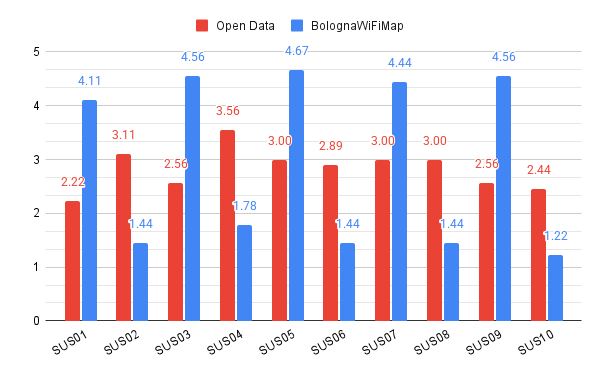
\includegraphics[width=\textwidth]{sus_avg_values_legend}
    \caption[Valori medi per ciascuna domanda del questionario SUS]{Valori medi per ciascuna domanda del questionario SUS. In rosso, quelli relativi al sito degli Open Data. In blu, quelli su BolognaWiFiMap.}
    \label{fig:sus_avg_values}
\end{figure}

\subsection{Valutazione dei risultati complessivi}
Possiamo già notare dalla Tabella~\ref{tab:sus_avg_values} come complessivamente BolognaWiFiMap batta gli Open Data su tutte le possibili metriche, a cominciare da un punteggio SUS quasi doppio. Sia nelle domande pari, che nelle domande dispari, la differenza tra media e mediana è molto piccola, segno di un insieme di dati piuttosto consistenti e senza particolari \textit{outliers}. Questa affermazione è ulteriormente supportata, per entrambe le tipologie di domanda, da una deviazione standard (abbastanza) piccola, che indica una bassa dispersione dei dati.

In particolare, diventa evidente come il valore medio e mediano delle domande dispari (positive) relativo a BolognaWiFiMap sia molto più elevato rispetto a quello degli Open Data. Allo stesso modo, il valore medio e mediano delle domande pari (negative) di BolognaWiFiMap risulta essere più basso di quello sugli Open Data, seppur con un margine inferiore rispetto alle domande dispari. Possiamo facilmente vedere queste differenze in maniera grafica in Figura~\ref{fig:sus_avg_values}. Relativamente ai criteri di valutazione delle domande pari e dispari, seppur con vario margine, non esiste nessun caso in cui il sito degli Open Data abbia performato meglio di BolognaWiFiMap.

Notiamo comunque come, relativamente alle categorie di domande pari e dispari, il sito degli Open Data abbia ottenuto una varianza maggiore nelle risposte rispetto a BolognaWiFiMap, indicando opinioni leggermente più contrastanti. Ciò è riscontrabile dal valore maggiore della deviazione standard, specialmente nelle domande pari. Questo ci fa pensare che ciascun utente abbia criteri di usabilità differenti, che diventano particolarmente evidenti quando si tratta di giudicare un sito non propriamente facile da utilizzare. D'altro canto, gli utenti sono stati più concordi nel giudizio di BolognaWiFiMap, cosa visibile sempre dalla deviazione standard.

\subsection{Risultati per ciascun utente}
Se complessivamente possiamo già decretare BolognaWiFiMap come sito avente l'usabilità migliore, non possiamo ancora trarre conclusioni relative alle preferenze di ciascun singolo utente. Andiamo quindi a vedere i risultati che ogni persona ha ottenuto nel questionario SUS relativo a entrambi i siti, in Tabella~\ref{tab:sus_scores}.

\begin{center}
    \begin{table}[H]
        \centering
        \begin{tabularx}{\textwidth}{|
            >{\hsize=0.5\hsize}X|
            >{\hsize=0.5\hsize}X|
            X|
            X|}
            \hline
            \multicolumn{4}{|c|}{\textbf{Confronto risultati SUS}} \\
            \hline
            \textbf{Utente} & \textbf{Età} & \textbf{Open Data} & \textbf{BolognaWiFiMap} \\
            \hline
            U01 & 24 & 22.5 & 97.5 \\
            U02 & 23 & 42.5 & 100 \\
            U03 & 23 & 60.0 & 75.0 \\
            U04 & 24 & 62.5 & 90.0 \\
            U05 & 23 & 27.5 & 75.0 \\
            U06 & 26 & 82.5 & 85.0 \\
            U07 & 24 & 25.0 & 97.5 \\
            U08 & 25 & 67.5 & 70.0 \\
            U09 & 30 & 22.5 & 97.5 \\
            \hline
            \multicolumn{2}{|X|}{\textbf{Punteggio medio}} & \textbf{45.8} & \textbf{87.5} \\
            \hline
            \multicolumn{2}{|X|}{\textbf{Mediana}} & 42.5 & 90.0 \\
            \hline
            \multicolumn{2}{|X|}{\textbf{Dev. Std.}} & 22.8 & 11.7 \\
            \hline
            \multicolumn{2}{|X|}{\textbf{\( \rho \) di Spearman}} & 0.0693 & 0.00 \\
            \hline
        \end{tabularx}
        \caption[Punteggi ottenuti dagli utenti nel questionario SUS]{Punteggi ottenuti dagli utenti nel questionario SUS. Viene quindi calcolato il punteggio medio complessivo, insieme a mediana, deviazione standard, e coefficiente di correlazione \( \rho \) di Spearman.}
        \label{tab:sus_scores}
    \end{table}
\end{center}

Anche qui notiamo chiaramente come nessun utente abbia mostrato una netta preferenza per il sito degli Open Data, seppur in due casi BolognaWiFiMap abbia ottenuto solo un leggerissimo vantaggio. Questo diventa particolarmente facile da vedere in maniera grafica dalla Figura~\ref{fig:sus_scores}.

Come prima, la media dei punteggi complessivi non si discosta molto dalla mediana, in linea con quanto è avvenuto per ciascuna risposta in Tabella~\ref{tab:sus_avg_values}, quindi l'insieme di dati è piuttosto consistente e non presenta particolari \textit{outliers}.

La deviazione standard, anche in questo caso, è maggiore per gli Open Data rispetto che a BolognaWiFiMap, segno di una più grande varianza tra le risposte e quindi di opinioni leggermente più contrastanti.

Per valutare la relazione tra l'età degli utenti e la percezione dell'usabilità, abbiamo utilizzato il coefficiente di correlazione \( \rho \) di Spearman , in quanto a differenza di quello di Pearson \( r \), non assume una distribuzione normale e misura la correlazione monotona tra due variabili. Di conseguenza è più adatto per piccoli campioni di dati e per relazioni non necessariamente lineari, come nel nostro caso.

Il coefficiente di correlazione di Spearman ( \( \rho \) ) è calcolato utilizzando la seguente formula:
\begin{equation}
    \rho = 1 - \frac{6 \sum d_i^2}{n(n^2 - 1)}
\end{equation}

I risultati ottenuti indicano che non esiste alcuna correlazione significativa tra l'età degli utenti e i punteggi SUS, suggerendo quindi che la percezione dell'usabilità dell'applicazione sia indipendente dall'età.


\[
d_i = R(x_i) - R(y_i)
\]

\[
d_i^2 = (R(x_i) - R(y_i))^2
\]

\[
R(x_i) = \text{Rango di } x_i \quad \text{(posizione di } x_i \text{ nella lista dei valori } x_1, ..., x_n \text{)}
\]

\[
R(y_i) = \text{Rango di } y_i \quad \text{(posizione di } y_i \text{ nella lista dei valori } y_1, ..., y_n \text{)}
\]

\begin{figure}[H]
    \centering
    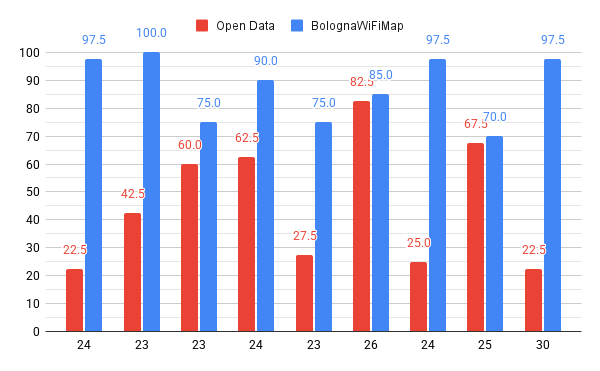
\includegraphics[width=\textwidth]{sus_scores_legend}
    \caption[Punteggi ottenuti nel questionario SUS]{Punteggi ottenuti dagli utenti nel questionario SUS, evidenziando l'età di ciascun utente in ascissa. In rosso, quelli relativi al sito degli Open Data. In blu, quelli su BolognaWiFiMap.}
    \label{fig:sus_scores}
\end{figure}